This chapter introduces and reviews general concepts of the wastewater treatment, machine learning techniques for regression.

\section{Wastewater Treatment}
\label{s:First-Background-Topic}

Provide background information that will help potential readers to understand your research. It is up to you to decide the volume and content of this chapter.

At the time you start writing your thesis you have probably already published novel works and become an expert in your field of research. You may find it difficulty to assume the perspective of a less experienced reader.

Your potential audience is predominately academic and works on tangentially related things. Thus, you may assume that a typical reader has successfully completed all compulsory undergraduate-degree subjects for a related degree. For example, if you do a PhD in computer science or a related discipline, you may assume that the reader knows what the difference between the declarative and imperative programming paradigm is, or what the difference between a linked-list and a tree is.

\section{Machine Learning}
\label{s:Second-Background-Topic}

Machine Learning is an area of the Artificial Intelligence where a computer is programmed to learn form data [A quick Review]. In 1959 Arthur Samuel defined the Machine Learning as \textbf{the field of study that gives the computers the ability to learn without being explicitly programmed}. Almost 40 years later, Tom Mitchell described Machine Learning as follows: \textbf{A computer program is said to learn from experience E with respect to some task T and some performance measure P, if its performance on T, as measured by P, improves with experience E.}

%\cite{raza_cinquergrana_2018}

\begin{figure}[t]
\centering
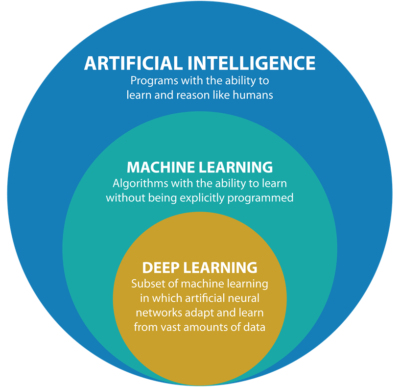
\includegraphics[width=8cm]{figures/AI-ML-DL.png}
\caption{AI, ML, DL}
\label{f:AI}
\end{figure}

\section{Deep Learning}
\label{s:Second-Background-Deep-Learning}

\begin{figure}[t]
\centering
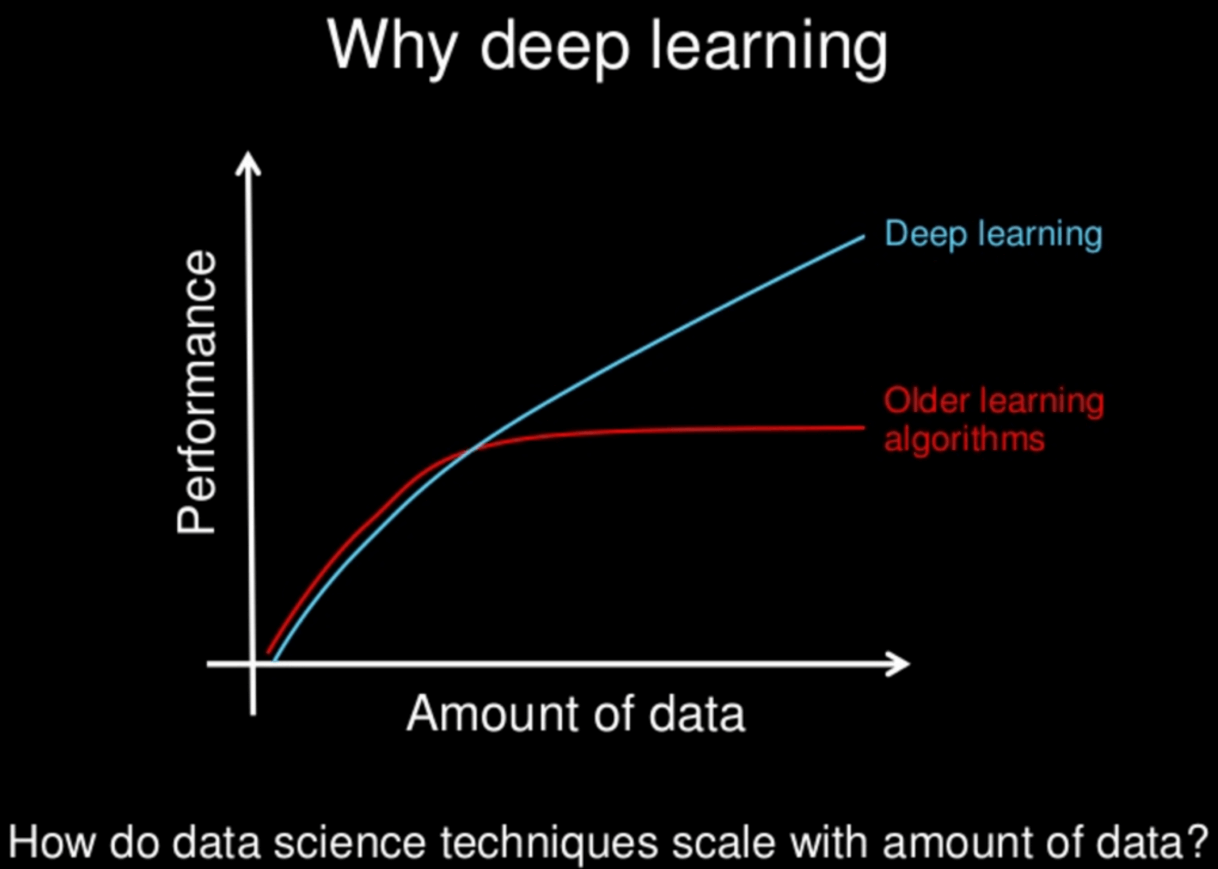
\includegraphics[width=8cm]{figures/MlvsDL-data-amount.png}
\caption{ML vs DL}
\label{f:ML-vs-DL}
\end{figure}

\section{Evaluation Metrics}
\label{sec:section_Example}
\subsection{Mean Absolute Percentage Error}
\subsubsection{Determination Coefficient}

\section{Summary}
\label{s:Background-Summary}

The final section of each chapter should summarize the chapter. In comparison to the chapter, the summary should be short ($\frac{1}{2}$ to $2$ pages is normal).

